\chapter{Introducción}

\section{Reseña de la Empresa}
\subsection{Historia}
El Laboratorio de Sistemas Espaciales (SETECLab) del Instituto Tecnológico de Costa Rica fue creado en Julio de 2017 para generar proyectos y programas con socios nacionales e internacionales con el propósito de desarrollar la ciencia y tecnología en el campo aeroespacial en Costa Rica.

Se identificaron las necesidades y fortalezas del país y se decidió iniciar un programa de pequeños satélites para monitoreo ambiental. El programa inicia con el satélite del proyecto Irazú, conocido como Batsú-CS1, el que fue el primer satélite Centroamericano. Hoy en día el programa continúa con el satélite GWSat, este último es liderado por la Universidad George Washington mientras que SETECLab se encarga de la red de sensores en tierra y el sistema de navegación.

\subsection{Misión}
Somos un laboratorio de ingeniería espacial enfocado en el desarrollo de proyectos y programas con socios nacionales e internacionales para el desarrollo de la ciencia y tecnología en el campo de la ingeniería en Costa Rica.

\subsection{Visión}
La visión del SETECLab es liderar la creación de capacidades en ingeniería espacial en Costa Rica.

\section{Planteamiento del Problema}
Existe la necesidad de diseñar e implementar una arquitectura de control térmico de las GRT. Estas son utilizadas en el segmento terrestre de las misiones espaciales que contemplan mediciones de variables ambientales en tierra.

Los equipos de las estaciones remotas deben protegerse del ambiente, para ello se instalan en gabinetes a prueba de polvo y humedad, esto limita la disipación de calor en el ambiente y hace necesario una solución de control termo mecánica no trivial. Además, existe una limitación energética de la GRT que obliga a que el control térmico sea pasivo, o bien, su consumo de potencia sea muy bajo.

\subsection{Problema a resolver}
Como parte de la nueva misión de investigación espacial GWSat, se requiere instalar una unidad de enlace satelital en los humedales del Parque Nacional Palo Verde.  Esta unidad recibe los datos recolectados por una red de sensores colocados en los humedales aledaños. Los datos incluyen batimetría del humedal; una vez consolidados estos datos, son transmitidos al satélite, por medio de un radio transmisor en órbita para la recolección de los datos.

Se ha comprobado de forma experimental que el radiotransmisor se puede sobrecalentar hasta fallar durante su operación normal. Esto se debe a que disipa grandes cantidades de potencia y se debe colocar en un gabinete cerrado.

Se espera que este fenómeno sea aún más severo en la ubicación final de la estación pues los datos de la estación meteorológica del Parque Nacional Palo Verde indican que la temperatura promedio de la zona es de \SI{30}{\celsius}.

\section{Objetivo General}
Diseñar un sistema modular que garantice la estabilidad térmica de los componentes electrónicos para la estación remota de Palo Verde.

\section{Objetivos Específicos}
\begin{enumerate}
    \item Realizar modelos cuantitativos que describan el comportamiento térmico de la estación remota. 
    \item Diseñar el sistema termo-mecánico para la estación remota de Palo Verde.
    \item Diseñar las interfaces entre los elementos de disipación de calor, el equipo electrónico y la estructura de la estación.
\end{enumerate}

\section{Justificación}
Es de vital importancia que dicho sistema funcione de manera correcta para garantizar la transmisión de los datos para la misión científica. Lo cual no puede ser posible si se alcanza temperaturas de operación que provocan el incorrecto funcionamiento del radio transmisor, incluso se corre el riesgo de incurrir en un daño físico a los dispositivos electrónicos.

Además, la GRT debe garantizar la protección contra el polvo y el ingreso de insectos. Por lo que la estación  contendrá los dispositivos electrónicos en un gabinete cerrado, la cual dependiendo de sus características geométricas y físicas, puede contribuir con la acumulación de calor dentro de la estación y empeorar las condiciones a las que el radio transmisor se ve sometido.

La misión científica consistirá en el monitoreo de las condiciones ambientales de los humedales del Parque Nacional de Palo Verde en Guanacaste para determinar el impacto climático en los mismos; lo que implica que la institución tiene a cargo la tarea de diseñar todo el sistema de recolección de datos, establecer el enlace satelital y realizar el procesamiento de datos. \cite{1} Por lo que, el presente proyecto se enfoca en mantener las condiciones idóneas de operación para el establecimiento del enlace con el satélite en órbita.

\section{Viabilidad}
Para la realización de este proyecto se cuenta con el apoyo del Laboratorio de Sistemas Espaciales del Instituto Tecnológico de Costa Rica por lo que se tiene acceso a los recursos del mismo; además se espera contar con la posibilidad de utilizar el Laboratorio DELTA de la escuela de ingeniería electromecánica, para la realización de pruebas y experimentos. Por otra parte, se contará con el acceso a equipo especializado de medición que permite el perfilado y validación de características del sistema.

A nivel de software, se manejan distintas herramientas de diseño estructural y electromecánico, además de la posibilidad de utilizar herramientas computacionales ya sea con licencias institucionales o bien licencias para estudiantes.

Por otra parte, al proyecto tiene una componente investigativa importante y se realiza dentro de la misma institución por lo tanto se puede contar con la colaboración de profesionales en diversas áreas y convertirse en un recurso de retroalimentación importante para el desarrollo del proyecto.

\section{Antecedentes del Proyecto}
\subsection{Estudio del Problema a Resolver}
La misión espacial Irazú tuvo como principales objetivos demostrar la capacidad de desarrollo de proyectos espaciales en Costa Rica, así como realizar la misión científica en la plantación Gmelina Arborea Roxb ubicada en Los Chiles, Alajuela, Costa Rica; para lo cual se definen tres elementos en su concepto de operaciones: \cite{2} 
\begin{itemize}
    \item Segmento de estación remota
    \item Segmento de vuelo
    \item Segmento en tierra
\end{itemize}

Para efectos del presente proyecto es de interés el segmento de estación remota, del cual en la siguiente figura se muestra la idea general de funcionamiento.

\begin{figure}[H]
\centering
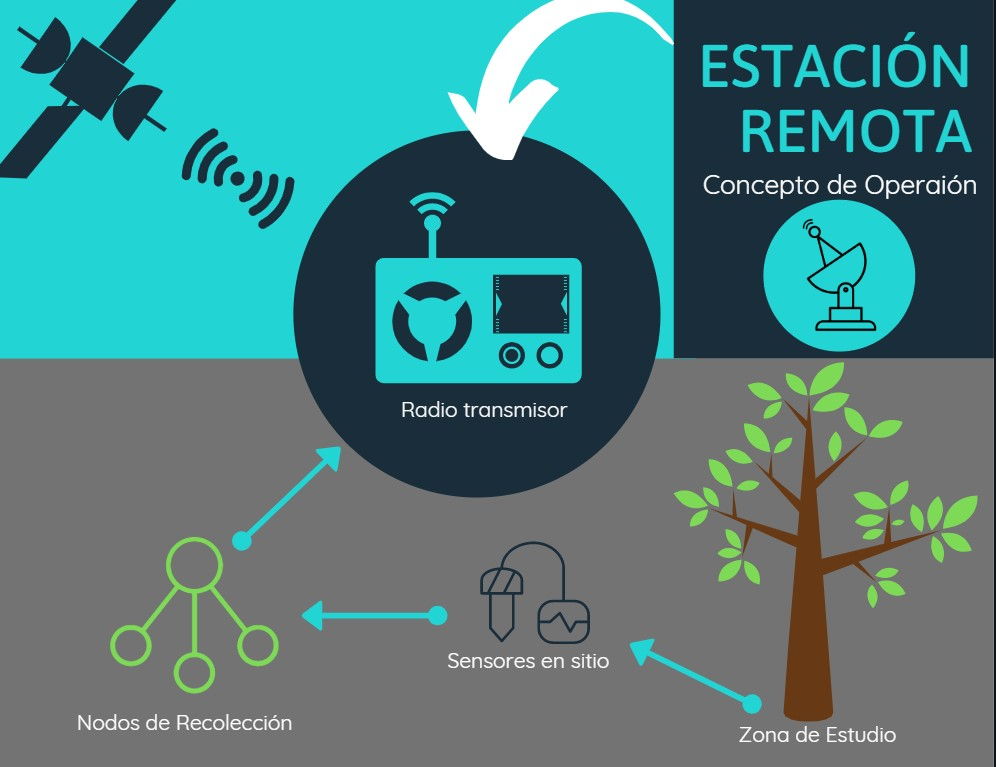
\includegraphics[scale=0.37]{Figuras/concepto_de_operacion_1.jpg}
\caption{Concepto de Operación para una estación Remota}
Elaboración Propia
\label{concepto de operacion}
\end{figure}

El concepto mostrado en la figura 1.1 fue el utilizado para la estación remota de la misión espacial Irazú; dicho concepto será el mismo para la nueva misión GWSat, esto incluye también, que el radio transmisor será reutilizado; por lo que conviene analizar los problemas operativos que surgieron en la misión Irazú como un antecedente, especialmente los que se dieron en la estación remota. Como antes se mencionó dentro de esta estación se encuentran los componentes electrónicos que hacen posible la transferencia de datos con el satélite, para el caso de la misión Irazú se identificaron tres problemas generales:

\begin{itemize}
    \item Ingreso de insectos y animales dentro del gabinete, por lo que no se garantizaba la protección de los componentes electrónicos internos.
    \item Incremento excesivo en la temperatura del radio transmisor.
    \item Fallos reiterados en la fuente de poder utilizada para el radio transmisor
    \item Pérdida de información debido al fallo general en la transmisión.
\end{itemize}

Como parte del problema, los responsables de la estación remota, identificaron como principal fuente de calor el radio transmisor; cabe resaltar que hasta ese momento, dentro del diseño inicial no se contempló ni se analizó la necesidad de un control térmico tanto para el radio como para el gabinete, por lo que para esta primera misión se encontraron desprovistos del mismo. Fuera de la información ya suministrada no se cuenta con documentación formal referente al estado operativo de la estación remota ni del radio transmisor durante la misión, ni reportes oficiales de reparaciones y mantenimientos realizados de los cuales se pudiera obtener información relevante para el proyecto.

\subsection{Requerimientos del Laboratorio}
En términos generales los requerimientos a nivel térmico-mecánico  por parte del laboratorio para la nueva misión GWSat se puede sintetizar en:
\begin{itemize}
    \item Determinar las condiciones térmicas del radio transmisor.
    \item Mantener el radio transmisor en condiciones operativas dentro del gabinete.
    \item Mantener una condición de estanqueidad en el gabinete de manera que no se permita el ingreso de polvo, agua, animales e insectos dentro del mismo.
    \item Considerar las condiciones climatológicas de Palo Verde en la determinación de los parámetros operativos de la estación.
    \item Poder introducir el radio transmisor dentro del gabinete desprovisto de su estructura termo-mecánica de fábrica.  
\end{itemize}

\section{Metodología}
\begin{figure}[h]
\centering
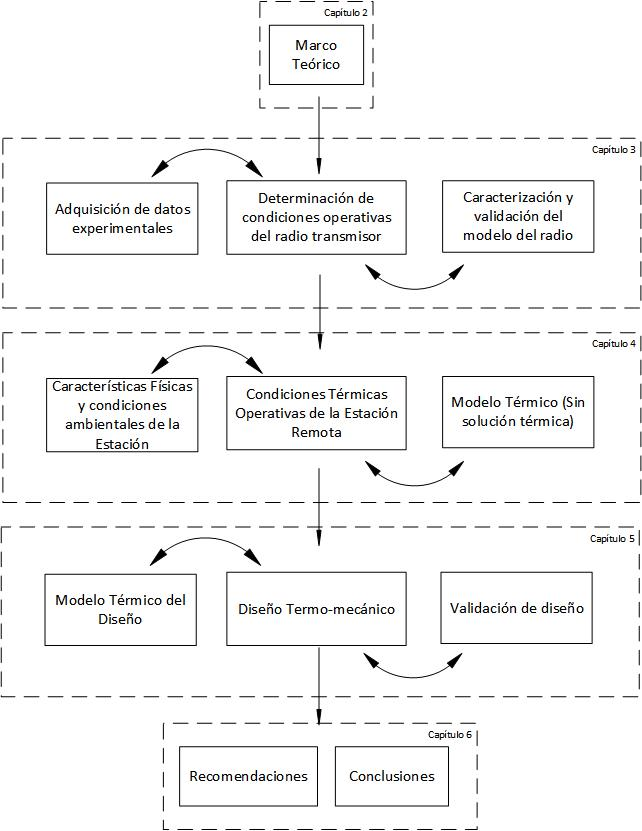
\includegraphics[width=0.9\linewidth]{Figuras/Metodologia.jpg}
\caption{Metodología de investigación}
Elaboración Propia
\label{Metodologia}
\end{figure}

Esta sección es una recopilación de lo más importante mediante los capítulos que definen los ejes centrales a seguir en el proyecto.

\begin{itemize}
    \item Capítulo 2: Hace referencia a toda la documentación técnica para la realización del diseño final.
    \item Capitulo 3: Se dedica exclusivamente al estudio del radio transmisor, con el fin de determinar su comportamiento térmico y la manera de poder analizarlo
    \item Capítulo 4: Involucra lo relacionado con la determinación de las condiciones térmicas, que determinarán los parámetros de diseño; y a las cuales la estación y el gabinete estarán sometidos.
    \item Capítulo 5: Se relaciona específicamente con el diseño en sí del control térmico, desde dos vertientes; la arquitectura de control térmico y la comparación con el modelo teórico propuesto.
    \item Capítulo 6: Dedicado a las conclusiones obtenidas del proceso de diseño, así como a las recomendaciones pertinentes sobre lo observado.
\end{itemize}

\subsection{Diseño de Investigación}

La investigación se define como experimental, ya que existe la posibilidad de la manipulación de la o las variables independientes haciendo variar por causa y efecto la variable dependiente \cite{meto}. En este caso el objetivo principal de la experimentación es la de caracterizar térmicamente el comportamiento del radio.

Al realizarle un análisis al funcionamiento del radio, además de las consultas realizadas a los encargados de la programación del mismo se identificaron tres posibles variables independientes que intervienen en la transmisión de datos por parte del radio hacia el satélite, que pudieran causar el aumento excesivo de la temperatura; sin embargo el criterio de selección y la especificación de dichas variables se realizará en el momento de definir el montaje del experimento.

\subsection{Enfoque de la Investigación}

Por las características propias del proyecto y de los objetivos planteados el enfoque de la investigación es cuantitativo por cumplir con las principales fases de este enfoque, las cuales se mencionan a continuación: \cite{meto}

\begin{itemize}
    \item Planteamiento del Problema.
    \item Revisión de la literatura y desarrollo del marco teórico.
    \item Desarrollo del diseño de investigación.
    \item Definición y selección de la muestra. 
    \item Recolección de datos.
    \item Análisis de datos.
    \item Reporte de Resultados.
\end{itemize}

\subsection{Definición del alcance de la investigación}

El principal  alcance de la investigación es de carácter exploratorio, ya que el tema no ha sido abordado antes  y actualmente se desconoce la magnitud del problema, al grado de que no se cuente con información necesaria para el planteamiento de una hipótesis. Sin embargo, una vez realizada la etapa exploratoria  referente al comportamiento térmico del radio, se pretende tener un alcance correccional donde se establezca el impacto de las variables independientes sobre el problema en estudio. \cite{meto}

